\documentclass[compress]{beamer}
%\documentclass[ignorenonframetext,handout]{beamer}
%\setbeamercovered{transparent}
%\usepackage[ISO 8859-1]{inputenc}
\usepackage{default}

% para usar figuras devemos acrescentar
\usepackage{graphicx}
%\usepackage{graphics}
%\DeclareGraphicsExtensions{.pdf,.png,.jpg}
%\DeclareGraphicsExtensions{.jpg, .eps}
%\DeclareGraphicsRule{.jpg}{eps}{.jpg}{`jpeg2ps -h -r 600 #1}
\usepackage{tikz}
%\usetikzlibrary{arrows,backgrounds,coordinatesystems,3d,shapes,plotmarks,automata,calendar,er,
%folding,matrix,mindmap,patterns,petri,plothandlers,topaths,trees} 
\usetikzlibrary{positioning}
%\usepgflibrary{decorations.pathreplacing}
\usetikzlibrary{decorations.pathreplacing}
\usetikzlibrary{decorations.pathmorphing}
\usetikzlibrary[patterns]
%\tikzstyle{every text node part}
%\usetikzlibrary{arrows,backgrounds,positioning,fit} 
\usetikzlibrary{calc}
% para gerar graficos no latex
\usepackage{pgfplots}
\pgfplotsset{compat=newest}

\usepackage{amsfonts}
\usepackage{amssymb}
\usepackage{amsmath}
\usepackage{MnSymbol}
\usepackage{amsmath,amsthm}
\usepackage[spanish]{babel}
\usepackage[utf8]{inputenc}
\usepackage{listings}
\usepackage{multirow, bigdelim}
\usepackage{hhline}
\usepackage{calc}



% \usepackage{algpseudocode}
% \usepackage{algorithmicx}
\usepackage[Algoritmo]{algorithm}
\usepackage[noend]{algorithmic}
\usepackage{float}
\usepackage[style=numeric,sorting=none,backend=biber]{biblatex}
%%%%
\usepackage{ragged2e}
\usepackage{chronosys}

\newcommand{\foreign}[1]{{\it #1}}

\setbeamertemplate{bibliography entry title}{}
\setbeamertemplate{bibliography entry location}{}
\setbeamertemplate{bibliography entry note}{}

\newcounter{saveenumi}
\newcommand{\seti}{\setcounter{saveenumi}{\value{enumi}}}
\newcommand{\conti}{\setcounter{enumi}{\value{saveenumi}}}

%\usepackage{shadethm}

%\definecolor{shadethmcolor}{rgb}{.75,.75,.75}

%\newshadetheorem{theorem}{\scshape Teorema}[chapter]
%\newtheorem{teorema}[theorem]{\scshape Teorema}
%\newtheorem{proposicao}[theorem]{\scshape Proposição}
%\newtheorem{corolario}[theorem]{\scshape Corolário}
%\newtheorem{lema}[theorem]{\scshape Lema}
%\newtheorem{definicao}[theorem]{\scshape Definição}
%\newtheorem{conjectura}[theorem]{\scshape Conjectura}
%\newtheorem{escolio}[theorem]{\scshape Escólio}
%\newtheorem{exemplo}[theorem]{\scshape Exemplo}
%\newtheorem{exemplos}[theorem]{\scshape Exemplos}
%\newtheorem{propriedade}[theorem]{\scshape Propriedade}

\renewcommand{\u}{{\bf u}}
\renewcommand{\v}{{\bf v}}
\renewcommand{\sin}{\operatorname{sen}}
\renewcommand{\tan}{\operatorname{tg}}
\providecommand{\cas}{\operatorname{cas}}
\providecommand{\mdc}{\mathrm{mdc}}
\providecommand{\f}{{\bf f}}

\newcommand{\ie}{\textit{i.e.}}
\newcommand{\eg}{\textit{e.g.}}
%\newcommand{\qed}{\hfill $\square$}

\renewcommand\Re{\operatorname{Re}}
\renewcommand\Im{\operatorname{Im}}

\providecommand{\x}{{\bf x}}
\providecommand{\y}{{\bf y}}
\providecommand{\w}{{\bf w}}
\providecommand{\f}{{\bf f}}
\providecommand{\q}{{\bf q}}
\providecommand{\bfa}{{\bf a}}
\providecommand{\bfb}{{\bf b}}
\providecommand{\bfc}{{\bf c}}
\providecommand{\bfd}{{\bf d}}
\providecommand{\bfe}{{\bf e}}
\providecommand{\bfs}{{\bf s}}
\providecommand{\bfz}{{\bf z}}
\providecommand{\zero}{{\bf 0}}
\providecommand{\spn}{\mathrm{span}}
\providecommand{\posto}{\mathrm{posto}}
\providecommand{\nul}{\mathrm{nul}}
\providecommand{\proj}{\mathrm{proj}}
\providecommand{\tr}{\mathrm{tr}}
\providecommand{\sgn}{\mathrm{sgn}}

\providecommand{\cov}{\mathrm{cov}}

\providecommand{\dilation}{\mathcal{D}}
\providecommand{\erosion}{\mathcal{E}}
\providecommand{\open}{\mathcal{O}}
\providecommand{\close}{\mathcal{C}}

\newcommand*{\Bhat}{\skew{3}{\hat}{B}}

\mode<presentation>
{
  \setbeamertemplate{background canvas}[vertical shading][bottom=white!10,top=blue!10]
%  \usetheme{Berkeley}
%  \usetheme{CambridgeUS}
%  \usetheme{Madrid}
  \usetheme{Warsaw}
  \usefonttheme[onlysmall]{structurebold}
  
  \setbeamertemplate{headline}{}
  
%   \setbeamercovered{invisible} % default
  \setbeamercovered{ transparent, again covered={\opaqueness{25}} } % =15%
%   \setbeamercovered{transparent=50}
%   \setbeamercovered{dynamic}

%   \setbeamercovered{again covered={\opaqueness<1->{25}}}
}

% copiado do site:
% http://latex-beamer-class.10966.n7.nabble.com/Covering-images-transparent-i-e-dimmed-figures-td1504
% . html
\usepackage{ifthen}

\makeatletter
\newcommand{\includecoveredgraphics}[2][]{
    \ifthenelse{\the\beamer@coveringdepth=1}{
        \tikz
            \node[inner sep=0pt,outer sep=0pt,opacity=0.15]
                {\includegraphics[#1]{#2}};
    }{
        \tikz
            \node[inner sep=0pt,outer sep=0pt]
                {\includegraphics[#1]{#2}};%
    }
} 

\newcommand{\thickhline}{%
    \noalign {\ifnum 0=`}\fi \hrule height 1pt
    \futurelet \reserved@a \@xhline
}

\makeatother

%\pgfdeclareimage[height=1.4cm]{logo_XIVsm}{semanauniversitaria}

%% put XIVsm logo in bottom left
%\setbeamertemplate{sidebar left}{
%%   \vfill%
 %  \rlap{\hskip0.0cm
  %       %\href{http://www.uece.br/semanauniversitaria}
   %      {\pgfuseimage{logo_XIVsm}}}
   %%\vskip2pt%
   %%\llap{\usebeamertemplate***{navigation symbols}\hskip0.1cm}%
   %%\vskip2pt%
%}

\DeclareMathOperator*{\argmax}{arg\,max}

% para que entre bien el título en el footer
\setbeamertemplate{footline}
{
  \leavevmode%
  \hbox{%
  \begin{beamercolorbox}[wd=.3\paperwidth,ht=2.25ex,dp=1ex,center]{author in head/foot}%
    \usebeamerfont{author in head/foot}\insertshortauthor
  \end{beamercolorbox}%
  \begin{beamercolorbox}[wd=.7\paperwidth,ht=2.25ex,dp=1ex,center]{title in head/foot}%
    \usebeamerfont{title in head/foot}\insertshorttitle\hspace*{3em}
    \insertframenumber{} / \inserttotalframenumber\hspace*{1ex}
  \end{beamercolorbox}}%
  \vskip0pt%
}

\setbeamertemplate{navigation symbols}{}

\title{Dise\~no de Interfaces de Usuario basado en Reconocimiento del Habla}
\author{Rodrigo Parra y Jorge Ram\'{i}rez}

\date{San Lorenzo, 2014}


\addbibresource{referencias.bib}
\begin{document}


\frame{\titlepage}

\frame{\tableofcontents}

\justifying
\section{Introducci\'on}

\begin{frame}{Introducci\'on}

\begin{figure}[H]
\centering

\includegraphics[width=0.7\linewidth]{./graphics/speech_intro.jpg}
\end{figure}


\end{frame}

\begin{frame}{Objetivos}
\begin{itemize}
    \uncover<+->{\item Antecedentes Hist\'oricos}
    \uncover<+->{\item Estado del Arte}
    \uncover<+->{\item Proceso del Reconocimiento del Habla}
    \uncover<+->{\item Herramientas Disponibles}
    \uncover<+->{\item Implementaci\'on}
    \uncover<+->{\item Evaluaci\'on}
\end{itemize}
\end{frame}
\section*{Antecedentes del Reconocimiento del Habla}

\begin{frame}{Antecedentes del Reconocimiento del Habla}
    % \begin{itemize}
    %     \item 50s: Inicios del &aacute;rea de investigaci&oacute;n.
    %     \item 60s: Desarrollo del \emph{Dynamic Time Warping}.
    %     \item 70s: Publicaci&oacute;n de la teor&iacute;a de los modelos ocultos de Markov (HMM).
    %     \item 80s: Adopci&oacute;n del modelo estad&iacute;stico. %Mencionar N-gramas!
    %     \item $&gt;$ 90s: Llegada del reconocimiento del habla al usuario com&uacute;n.
    %     \item 2016-2019: Meseta de productividad seg&uacute;n Gartner.
    % \end{itemize}

    % \begin{chronology}[5]{1950}{2019}{\textwidth}
    %     \event{1950}{Inicios del \'area de investigaci\'on.}
    %     \event{1960}{Desarrollo del \emph{Dynamic Time Warping}.}
    %     \event{1970}{Publicaci\'on de la teor{\'\i}a de los modelos ocultos de Markov (HMM).}
    %     \event{1980}{Adopci\'on del modelo estad{\'\i}stico.}
    %     \event[1990]{2014}{Llegada del reconocimiento del habla al usuario com\'un.}
    %     \event[2016]{2019}{Meseta de productividad seg\'un Gartner.}
    % \end{chronology}

\startchronology[startyear=1950,stopyear=2020,color=blue]
  \uncover<8-8>{\chronoperiode[textdepth=20pt, startdate=false, stopdate=false, colorbox=lightgray]{2016}{2020}{\emph{Gartner}}}
  % \chronoperiode{1990}{2014}{Llegada del reconocimiento del habla al usuario com\'un.}
  \uncover<7-8>{\chronoevent[markdepth=100pt, colorbox=lightgray]{2008}{\emph{Google Voice Search}}}
  \uncover<6-8>{\chronoevent[markdepth=60pt, colorbox=lightgray]{2007}{\emph{Apple Siri}}}
  \uncover<4-8>{\chronoevent[markdepth=130pt, colorbox=lightgray]{1986}{N-Gramas}}
  \uncover<5-8>{\chronoevent[colorbox=lightgray]{1997}{\emph{Dragon Naturally Speaking}}}
  \uncover<3-8>{\chronoevent[markdepth=90pt, colorbox=lightgray]{1975}{Modelos Ocultos de Markov}}
  \uncover<2-8>{\chronoevent[markdepth=50pt, colorbox=lightgray]{1968}{\emph{Dynamic Time Warping}}}
  \uncover<1-8>{\chronoevent[colorbox=lightgray]{1952}{\qquad Inicia investigaci\'on.}}
\stopchronology

% \startchronology
% \chronoevent[markdepth=60pt]{1525}{Label B}
% \chronoevent{1500}{Label A}
% \stopchronology

\end{frame}
\section{Actualidad y Aplicaciones}

\begin{frame}{Actualidad y Aplicaciones}
El panorama actual del reconocimiento del habla se caracteriza por su aplicaci\'on
en diversos \'ambitos, algunos de los cuales se mencionan a continuaci\'on:

\begin{itemize}
	\item{\textbf{Medicina y Derecho:}}
    existen aplicaciones comerciales y trabajos de investigaci\'on enfocados a la transcripci\'on de registros 
    m\'edicos \cite{LaiMedSpeak1997, USATodayHospitals} y reportes legales \cite{FalavignaAutomatic2009, NuanceLegal}
	mediante reconocimiento del habla.

	\item{\textbf{Milicia:}}
	se destacan los trabajos de Beek \cite{BeekAn1977} y Weinstein \cite{WeinsteinOpportunities1991},
	en los cuales se clasifican las potenciales aplicaciones de tecnolog\'ias del habla en 
	cinco categor{\'\i}as: seguridad, mando y control, transmisi\'on de datos y comunicaci\'on, 
	procesamiento de voz distorsionada y aplicaciones para entrenamiento.
\end{itemize}
\end{frame}
\begin{frame}{Actualidad y Aplicaciones (2)}
\begin{itemize}
	\item{\textbf{Telefon\'ia:}}
	las aplicaciones de reconocimiento del habla buscan reducir los costos, como
	la automatizaci\'on de consulta de directorio, 
	o producir ganancias mediante nuevos modelos de servicio, como servicios bancarios
	y de servicios de reserva \cite{RabinerApplications1997}.

	\item{\textbf{Accesibilidad:}}
	las interfaces mediante voz poseen un gran potencial para usuarios con alg\'un tipo de discapacidad
	que les impida manejar apropiadamente el rat\'on y/o el teclado o visualizar la informaci\'on en el monitor.
	Varios ejemplos de este tipo de aplicaciones se mencionan en \cite{AnanthiSurvey2013}.
\end{itemize}
\end{frame}
\begin{frame}{Actualidad y Aplicaciones (3)}
\begin{itemize}
	\item{\textbf{Industria Automotriz:}}
	seg\'un \cite{Kirriemuir2003Speech}, el desarrollo de sistemas de reconocimiento del habla para autom\'oviles
	se divide en las siguientes \'areas: dispositivos manos libres, control
	de los dispositivos de navegaci\'on, interacci\'on con el sistema de control y sistemas de manejo por voz.

	\item{\textbf{Tel\'efonos Inteligentes e Interfaces Web:}}
	se destaca el surgimiento de los asistentes virtuales,
	como \emph{Google Now} \cite{GoogleNow} y \emph{Siri} \cite{AppleSiri}. Adem\'as,
	puede mencionarse la \emph{Web Speech API} \cite{GoogleWebSpeechAPI}, una propuesta de \emph{Google}
	a la \emph{W3C} que permite integrar reconocimiento y s\'intesis del habla a las aplicaciones web.
\end{itemize}
\end{frame}
\begin{frame}{Actualidad y Aplicaciones (4)}
\begin{itemize}
	\item{\textbf{Videojuegos y Dom\'otica:}}
	existen juegos comerciales que interactuan con el usuario
	mediante la voz, como \emph{Say-N-Play}\cite{SayNPlay}. En el caso de la dom\'otica, 
	est\'an disponibles productos que permiten controlar los artefactos del hogar mediante la voz, 
	como \emph{HAL} \cite{HAL}.
\end{itemize}
\end{frame}

\section{Proceso B\'asico del Reconocimiento del Habla}

\begin{frame}{Proceso B\'asico del Reconocimiento del Habla (1/8)}
\uncover<1-2>{
\begin{quote}
\emph{La b\'usqueda de la oraci\'on m\'as probable W perteneciente al lenguaje L, dada la entrada ac\'ustica 0.}
\end{quote}
}

\uncover<2-2>{
\begin{align}
\hat{W} = \argmax_{W \in L} \overbrace{P(O|W)}^\text{M. ac\'ustico}\overbrace{P(W)}^\text{M. de lenguaje}
\label{eq:asrFundamental}
\end{align}
}
\end{frame}

\begin{frame}{Proceso B\'asico del Reconocimiento del Habla (2/8)}

\begin{figure}[H] 
\centering
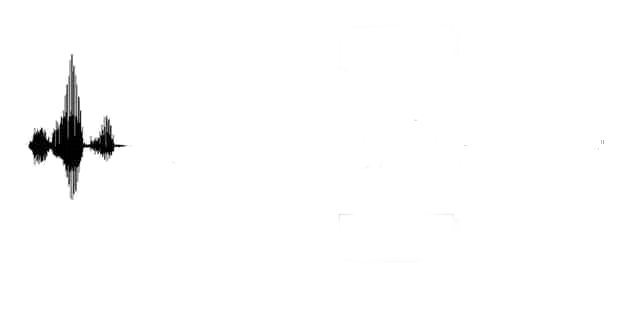
\includegraphics[width=0.8\textwidth]{./graphics/proceso_00.png}
\caption{Proceso del reconocimiento del habla. Traducido a partir de \protect\cite{VerenichASR}.}
\label{figure:proceso}
\end{figure}
\end{frame}

\begin{frame}{Proceso B\'asico del Reconocimiento del Habla (2/8)}

\begin{figure}[H] 
\centering
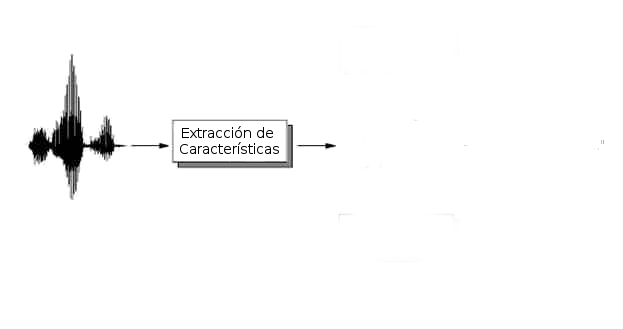
\includegraphics[width=0.8\textwidth]{./graphics/proceso_0.png}
\caption{Proceso del reconocimiento del habla. Traducido a partir de \protect\cite{VerenichASR}.}
\label{figure:proceso}
\end{figure}
\end{frame}

\begin{frame}{Proceso B\'asico del Reconocimiento del Habla (2/8)}

\begin{figure}[H]  
\centering
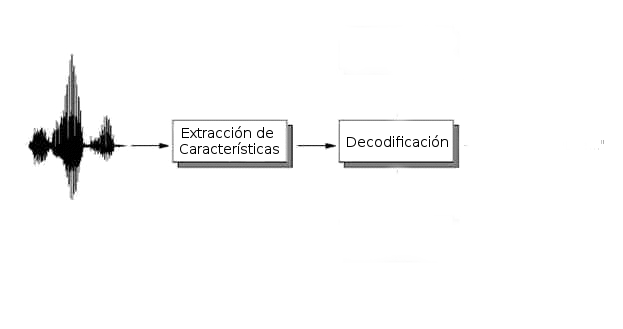
\includegraphics[width=0.8\textwidth]{./graphics/proceso_1.png}
\caption{Proceso del reconocimiento del habla. Traducido a partir de \protect\cite{VerenichASR}.}
\label{figure:proceso}
\end{figure}
\end{frame}

\begin{frame}{Proceso B\'asico del Reconocimiento del Habla (2/8)}

\begin{figure}[H] 
\centering
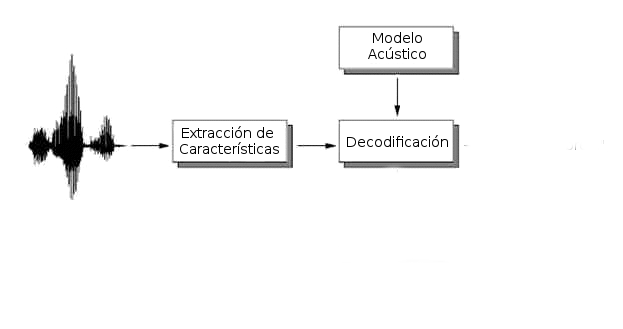
\includegraphics[width=0.8\textwidth]{./graphics/proceso_2.png}
\caption{Proceso del reconocimiento del habla. Traducido a partir de \protect\cite{VerenichASR}.}
\label{figure:proceso}
\end{figure}
\end{frame}

\begin{frame}{Proceso B\'asico del Reconocimiento del Habla (2/8)}

\begin{figure}[H] 
\centering
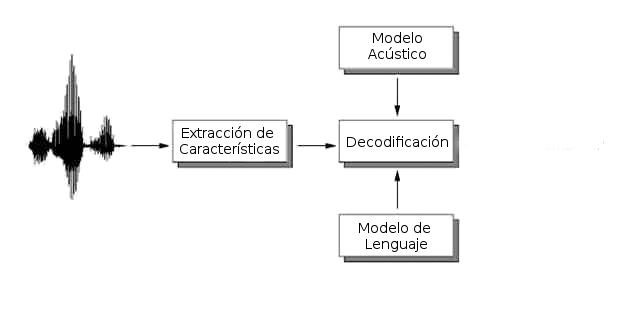
\includegraphics[width=0.8\textwidth]{./graphics/proceso_3.png}
\caption{Proceso del reconocimiento del habla. Traducido a partir de \protect\cite{VerenichASR}.}
\label{figure:proceso}
\end{figure}
\end{frame}

\begin{frame}{Proceso B\'asico del Reconocimiento del Habla (2/8)}

\begin{figure}[H] 
\centering
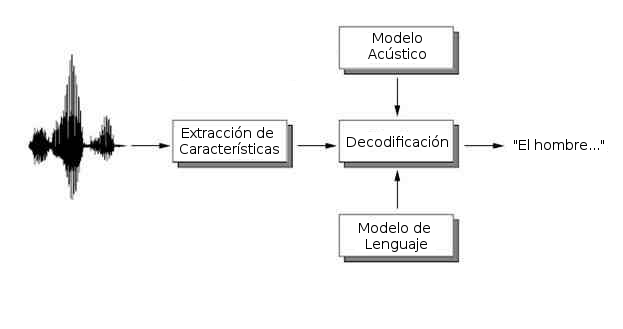
\includegraphics[width=0.8\textwidth]{./graphics/proceso.png}
\caption{Proceso del reconocimiento del habla. Traducido a partir de \protect\cite{VerenichASR}.}
\label{figure:proceso}
\end{figure}
\end{frame}
\begin{frame}{Proceso B\'asico del Reconocimiento del Habla (3/8)}
\framesubtitle{Fase 1: Extracci\'on de caracter{\'\i}sticas}
\uncover<1-2>{
\begin{figure}[H]
\centering
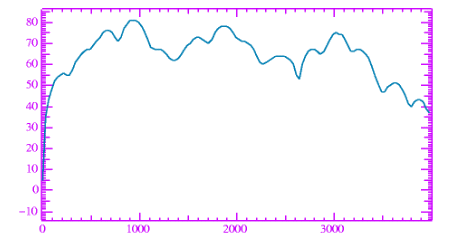
\includegraphics[width=0.4\linewidth]{./graphics/formants.png}
\caption{Representaci\'on del espectro en el cual pueden identificarse los picos espectrales o formantes 
\cite{Jurafsky}.}
\label{figure:formants}
\end{figure}
}

\uncover<2-2>{
\begin{figure}[H]
\centering
\only<2-2>{
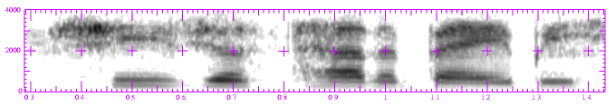
\includegraphics[width=0.7\linewidth]{./graphics/spectrogram.png}
\caption{Representaci\'on de un espectrograma, puede verse como una colecci\'on de espectros  ubicados uno despu\'es de otro \cite{Jurafsky}.}}
\label{figure:spectrogram}
\end{figure}
}
\end{frame}

\begin{frame}{Proceso B\'asico del Reconocimiento del Habla (4/8)}
\framesubtitle{Fase 1: Extracci\'on de caracter{\'\i}sticas}

\begin{figure}[H] 
\centering
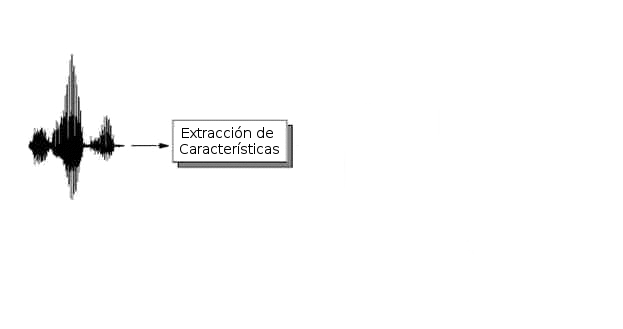
\includegraphics[width=0.8\textwidth]{./graphics/extraccion_0.png}
\caption{Fase de extracci\'on de caracter{\'\i}sticas. Gr\'afico basado en \cite{VerenichASR}.}
\label{figure:hmm}
\end{figure}
\end{frame}

\begin{frame}{Proceso B\'asico del Reconocimiento del Habla (4/8)}
\framesubtitle{Fase 1: Extracci\'on de caracter{\'\i}sticas}

\begin{figure}[H] 
\centering
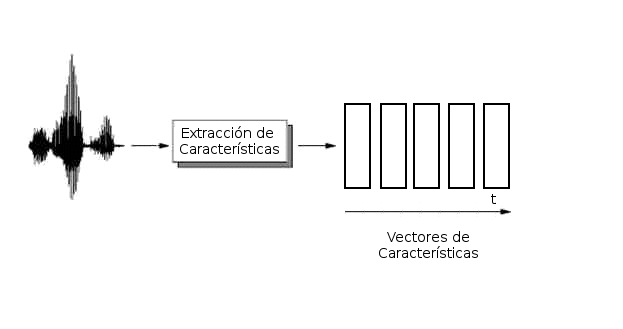
\includegraphics[width=0.8\textwidth]{./graphics/extraccion.png}
\caption{Fase de extracci\'on de caracter{\'\i}sticas. Gr\'afico basado en \cite{VerenichASR}.}
\label{figure:hmm}
\end{figure}
\end{frame}


\begin{frame}{Proceso B\'asico del Reconocimiento del Habla (5/8)}
\framesubtitle{Fase 2: Decodificaci\'on: Modelo de Lenguaje}
\uncover<1-3>{Probabilidad de ocurrencia de una secuencia de palabras $x_1,x_2,\ldots,x_n$ para un lenguaje dado.}
\vspace*{2\baselineskip}
\begin{itemize}
    \uncover<2-3>{\item Basado en N-Gramas
        \small \begin{equation*}
            \hspace*{-1.5cm} 
            p(\text{el, hombre, corre}) = p(el \mid \text{\textless} s\text{\textgreater}) \, 
            p(\text{\emph{hombre}} \mid el) \, p(corre \mid \text{\emph{hombre}}) \, 
            p(\text{\textless} /s\text{\textgreater} \mid corre)
        \end{equation*}}
        \vspace*{1\baselineskip}
        \uncover<3-3>{\item Basado en Gram\'atica
        \begin{bnf*}
            \bnfprod{pregunta}
            {\bnfts{Cu\'al} \bnfsp \bnfts{es} \bnfsp \bnfts{la}  \bnfpn{info} \bnfsp  \bnfts{en} \bnfsp \bnfpn{ciudad}} \\
            \bnfprod{info}
            {\bnfts{temperatura} \bnfor \bnfts{presi\'on atmosf\'erica} \bnfor \bnfts{hora}} \\
            \bnfprod{ciudad}
            {\bnfts{Par{\'\i}s} \bnfor \bnfts{Nueva York} \bnfor \bnfts{Roma}}
        \end{bnf*}}
    \end{itemize}
\end{frame}

\begin{frame}{Proceso B\'asico del Reconocimiento del Habla (6/8)}
\framesubtitle{Fase 2: Decodificaci\'on - Modelo Ac\'ustico}

\setbeamercovered{transparent}
\uncover<1-9>{Probabilidad de una entrada ac\'ustica $O$ dada una secuencia de \mbox{palabras $W$.}}
\begin{columns}
\column{0.45\linewidth}
\onslide<2-9>{
\begin{itemize}
    \uncover<1-9>{\item Modelos Ocultos de Markov}
        \begin{itemize}
                \uncover<4-9>{\item Estados: $S$}
                \uncover<5-9>{\item Observaciones: $V$}
                \uncover<6-9>{\item Probabilidad inicial: $\pi$}
                \uncover<7-9>{\item Probabilidad de transici\'on: $a$}
                \uncover<8-9>{\item Probabilidad de observaci\'on: $b$}
        \end{itemize}
    \uncover<9-9>{\item Diccionario Fon\'etico}
\end{itemize}
}

\column{0.55\linewidth}
\begin{figure}[H]
\centering
\uncover<3-9>{
\only<3-9>{
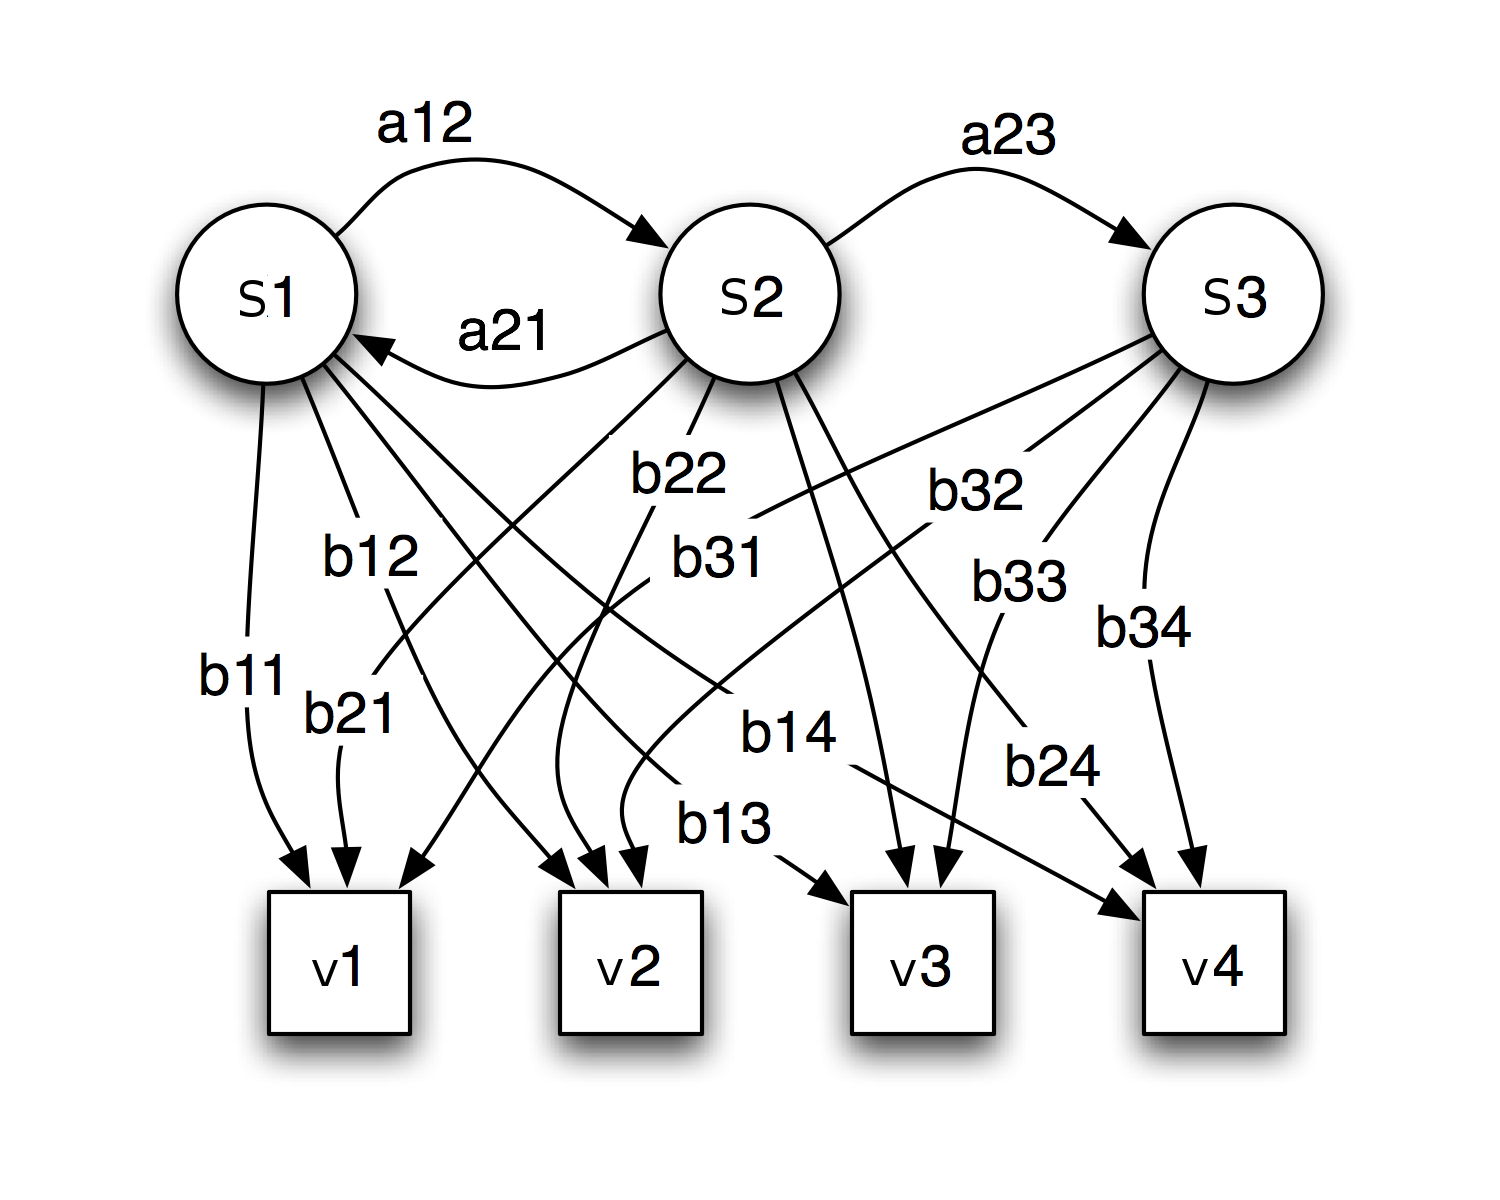
\includegraphics[width=1\textwidth]{./graphics/hmm.png}
\caption{Representaci\'on de un modelo oculto de Markov.}}}
\label{figure:esquema-herramientas}
\end{figure}
\end{columns}


\end{frame}

\begin{frame}{Proceso B\'asico del Reconocimiento del Habla (7/8)}
\framesubtitle{Fase 2: Decodificaci\'on - B\'usqueda}

\setbeamercovered{transparent}
\begin{columns}
\column{0.30\linewidth}
\onslide<1-3>{
\begin{itemize}
    \uncover<2-3>{\item Algoritmo de Viterbi.}
    \uncover<3-3>{\item Algoritmo A*.}
\end{itemize}
}

\column{0.7\linewidth}
\begin{figure}[H]
\centering
\uncover<1-3>{
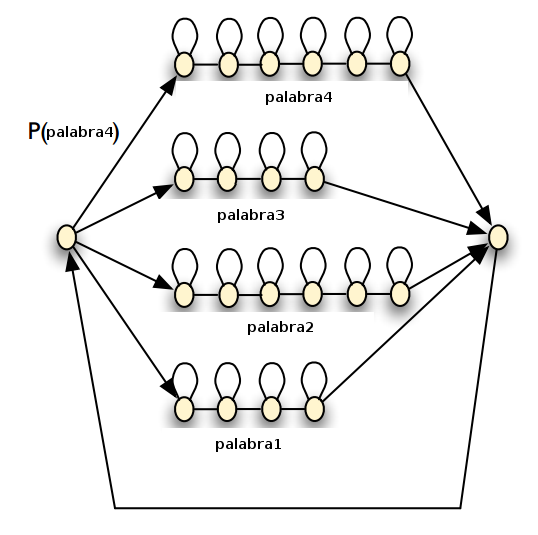
\includegraphics[width=0.8\textwidth]{./graphics/espacio.png}
\caption{Espacio de b\'usqueda para un lenguaje simple de cuatro palabras. Traducido a partir de \cite{RenalsSearch}.}}
\label{figure:espacio-busqueda}
\end{figure}
\end{columns}


\end{frame}

\begin{frame}{Proceso B\'asico del Reconocimiento del Habla (8/8)}
\framesubtitle{Fase 2: Decodificaci\'on}
\begin{figure}[H] 
\centering
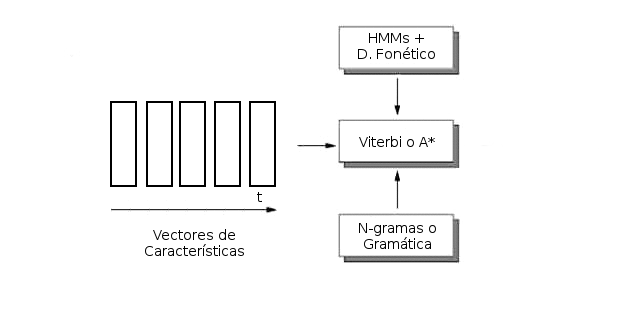
\includegraphics[width=0.8\textwidth]{./graphics/decodificacion0.png}
\caption{Fase de decodificaci\'on. Gr\'afico basado en \cite{VerenichASR}.}
\label{figure:decoding}
\end{figure}
\end{frame}


\begin{frame}{Proceso B\'asico del Reconocimiento del Habla (8/8)}
\framesubtitle{Fase 2: Decodificaci\'on}
\begin{figure}[H] 
\centering
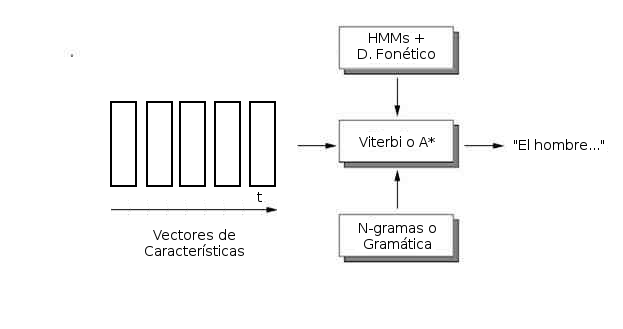
\includegraphics[width=0.8\textwidth]{./graphics/decodificacion.png}
\caption{Fase de decodificaci\'on. Gr\'afico basado en \cite{VerenichASR}.}
\label{figure:decoding}
\end{figure}
\end{frame}

\section{Tecnolog\'ias y Herramientas}

\begin{frame}{Tecnolog\'ias y Herramientas}
\setbeamercovered{transparent}
\begin{columns}
\column{0.30\linewidth}
\visible<1-3>{
\begin{itemize}
    \uncover<+->{\item Clasificaci\'on}
    \uncover<+->{\item Criterios}
\end{itemize}
}
\column{0.7\linewidth}
\invisible<1-2>{\begin{figure}[H]
\centering
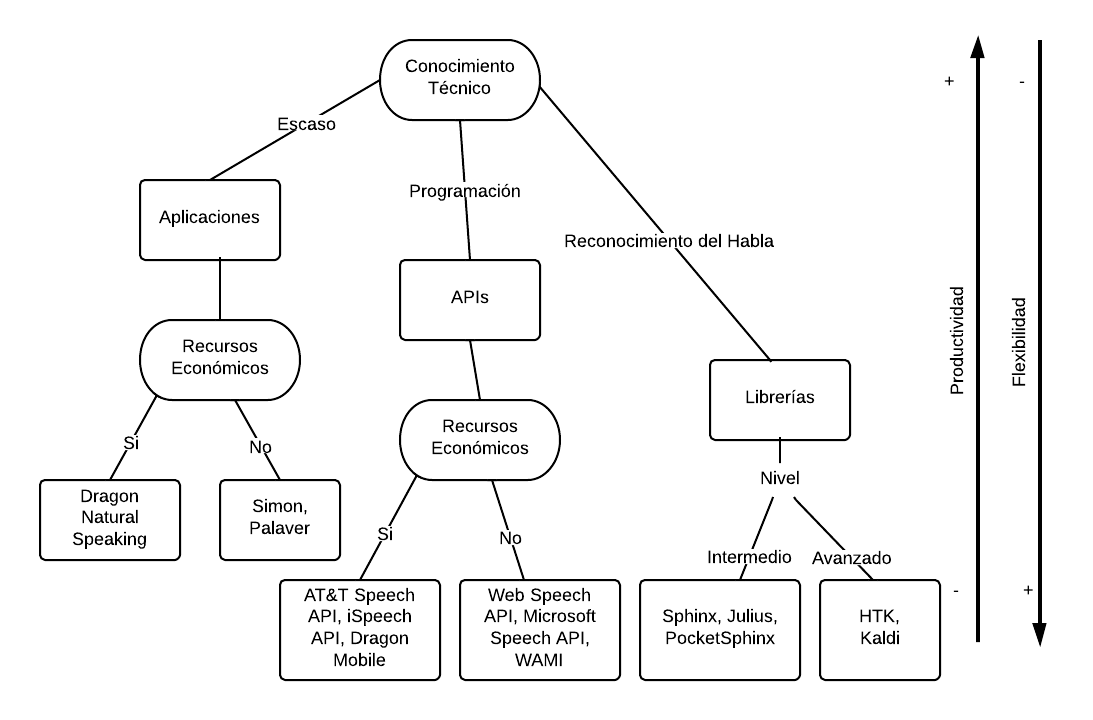
\includegraphics[width=1.1\linewidth]{./graphics/esquema-herramientas.png}
\caption{Esquema de la clasificaci\'on de tecnolog{\'\i}as y herramientas}
\label{figure:esquema-herramientas}
\end{figure}}
\end{columns}
\end{frame}
\section{Definici\'on del Problema}

\begin{frame}{Definici\'on del Problema (1/2)}

\begin{table}[H]
\centering
\footnotesize
\begin{tabular}{|p{2.5cm}|p{7cm}|}
\hline
Desafíos  &   Oportunidades \\
\hline
\uncover<2-7>{ Transitoriedad } &       \uncover<5-7>{ Usuarios con discapacidades }  \\
\uncover<3-7>{ Invisibilidad } & \uncover<6-7>{ Usuarios en situaciones de manos y vista ocupadas }\\
\uncover<4-7>{ Asimetr{\'\i}a }  &  \uncover<7-7>{ Usuarios sin acceso a un teclado o monitor }     \\
\hline  
\end{tabular}
\label{sec:tabla-resumen-prueba}
\end{table}

% \uncover<+->{Desaf{\'\i}os de las interfaces mediante voz\cite{GabrielVoice2007}:}

% \begin{itemize}
%     \vfill \item<+->{ Transitoriedad }
%     \vfill \item<+->{ Invisibilidad }
%     \vfill \item<+->{ Asimetr{\'\i}a }
% \end{itemize}

% \uncover<+->{Presentan un gran potencial para \cite{NielsenVoice2003}:}

% \begin{itemize}
%     \vfill \item<+->{ Usuarios con discapacidades }
%     \vfill \item<+->{ Usuarios en situaciones de manos y vista ocupadas }
%     \vfill \item<+->{ Usuarios sin acceso a un teclado o monitor }
% \end{itemize}

\end{frame}

\begin{frame}{Definici\'on del Problema (2/2)}
\uncover<+->{Investigaci\'on de la influencia de factores como:}

\begin{itemize}
    \vfill \item<+->{Dominio.}
    \vfill \item<+->{Tama\~no del lenguaje.}
    \vfill \item<+->{Longitud de los comandos.}
    \vfill \item<+->{Duraci\'on de la interacci\'on.}
\end{itemize}

\end{frame}
\section{Soluci\'on Propuesta}

\begin{frame}{Soluci\'on Propuesta}
\end{frame}

\section{Evaluaci\'on}

\begin{frame}{Evaluaci\'on}
\framesubtitle{Metodolog\'ia}

\begin{itemize}
    \item 12 estudiantes.
    \item Laboratorio de Inform\'atica de la FPUNA.
    \item 2 semanas.
\end{itemize}

Las características de cada sesión son:
\begin{itemize}
    \item Duración: aproximadamente una hora
    \item Participantes:
        \begin{itemize}
            \item Usuario
            \item Facilitador
            \item Observador
        \end{itemize}
    \item Fases:
        \begin{itemize}
            \item Test de Memoria
            \item Entrenamiento
            \item Tareas
            \item Encuesta de Usabilidad
            \item Recopilación y Análisis de Datos
        \end{itemize}   
\end{itemize}
\end{frame}


\begin{frame}{Evaluaci\'on (2)}
\framesubtitle{Análisis de Datos}
    \begin{itemize}
        \item Memoria del Usuario: Test de Memoria ($M$)
        \item Correctitud de la Aplicación
            \begin{itemize}
                \item Tasa de Acierto ($A$)
                \item Tasa de Error de Comandos ($E_1$)
            \end{itemize}
        \item Error Humano
            \begin{itemize}
                \item Tasa de Error Humano ($E_2$)
                    \begin{itemize}
                        \item Tasa de Error por Longitud del Comando
                        \item Tasa de Error por Nivel Contextual del Comando
                        \item Tasa de Error por Comando
                        \item Distribuci\'on del Error Humano por Etapas de la Sesi\'on 
                    \end{itemize}
                \item Cantidad de Errores ($E_3$)
            \end{itemize}
        \item Eficiencia
            \begin{itemize}
                \item Duración de Tareas Uno y Dos ($T_{1+2}$)
                \item Duración de Tareas Tres y Cuatro($T_{3+4}$)
                \item Cantidad de Comandos Utilizados ($U$)
                \item Correctitud de la Tarea Cuatro ($C$)
            \end{itemize}
        \item Satisfacción del Usuario: Encuesta de Usabilidad
    \end{itemize}
\end{frame}
\section{Resultados Obtenidos}

\begin{frame}{Resultados Obtenidos}
\framesubtitle{Metodolog\'ia}

\begin{table}[H]
\centering
\footnotesize
\caption{Resumen de las variables de la prueba de usabilidad}
\begin{tabular}{|p{1.2cm}|p{2.4cm}|}
\hline
M\'etrica  &   Promedio \\
\hline
$M$ &       12,75  palabras  \\
$A$  &      83,70 \%     \\
$E_1$ &     16,30 \%  \\
$E_2$  &    5,91  \%  \\
$T_{1+2}$ & 13,83  minutos  \\
$T_{3+4}$ & 18,35  minutos  \\
$E_3$ &     11,83  errores  \\
$C$ &       87,5   \%  \\
$U$ &       40.67  comandos  \\
\hline  
\end{tabular}
\label{sec:tabla-resumen-prueba}
\end{table}

\end{frame}

\begin{frame}{Resulados Obtenidos}
\framesubtitle{Correlaci\'on}
\begin{table}[H] 
\centering
\footnotesize
\begin{tabular}{|p{0.5cm}|p{0.75cm}|p{0.7cm}|p{0.75cm}|p{0.75cm}|p{0.75cm}|p{0.75cm}|p{0.75cm}|p{0.7cm}|p{0.75cm}|}
\hline
& $M$ &  $A$  &   $E_1$ &  $E_2$  &  $T_{1+2}$  & $T_{3+4}$     & $E_3$ & $C$ & $U$ \\
\hline
$M$       &  1     &  0,22  & -0,22  & \textbf{-0,38}  &  \textbf{-0,31}  &  \textbf{-0,42}  &  -0,29 & -0,08    &  -0,23 \\
$A$       &  0,22  &  1  &  -1  &  \textbf{0,51}  &  0,14  &  -0,09  &  \textbf{0,69}  &  \textbf{0,5}           &  \textbf{0,53} \\
$E_1$     &  -0,22 &  -1  &  1  &  \textbf{-0,51}  &  -0,14  &  0,09  &  \textbf{-0,69}  &  \textbf{-0,5}        &  \textbf{-0,53} \\
$E_2$     &  \textbf{-0,38} &  \textbf{0,51}  &  \textbf{-0,51}  &  1  &  \textbf{0,4}  &  0,23  &  \textbf{0,71}  &  0,29         &  0,35  \\
$T_{1+2}$ &  \textbf{-0,31} &  0,14  &  -0,14  &  \textbf{0,4}  &  1  &  \textbf{0,87}  &  \textbf{0,57}  &  -0,04        &  0,25 \\
$T_{3+4}$ &  \textbf{-0,42} &  -0,09  &  0,09  &  0,23  &  \textbf{0,87}  &  1  &  0,37  &  -0,16       &  0,2 \\
$E_3$     &  -0,29 &  \textbf{0,69}  &  \textbf{-0,69}  &  \textbf{0,71}  &  \textbf{0,57}  &  \textbf{0,37}  &  1  &  0,28        &  \textbf{0,52} \\
$C$       &  -0,08 &  \textbf{0,5}  &  \textbf{-0,5}  &  0,29  &  -0,04  &  -0,16  &  0,28  &  1        &  0,13 \\
$U$       &  -0,23 &  \textbf{0,53}  &  \textbf{-0,53}  &  \textbf{0,35}  &  0,25  &  0,2  &  \textbf{0,52}  &  0,13      &  1 \\
\hline
\end{tabular}
\caption{Coeficientes de correlaci\'on para las m\'etricas consideradas.}
\label{sec:tabla-correlacion}
\end{table}

\end{frame}

\begin{frame}{Resultados Obtenidos}
\framesubtitle{An\'alisis del Error Humano}
\begin{table}[H]
\centering
\footnotesize
\begin{tabular}{|p{1.2cm}|p{1.0cm}|p{1.0cm}|p{1.0cm}|p{1.0cm}|p{1.0cm}|}
\hline
    Sujeto & 2 & 3 & 4 & 5 & 6  \\
    \hline 
    Promedio & 6,96 & 5,68 & 7,46 & 14,81 & 42,11 \\
\hline
\end{tabular}
\caption{Tasa de error humano por longitud del comando.}
\label{sec:error-longitud}
\end{table}


\begin{table}[H]
\centering
\footnotesize
\begin{tabular}{|p{1.6cm}|p{1.6cm}|p{1.6cm}|p{1.6cm}|}
\hline
    Sujeto & General & Pista & Comp\'as \\
\hline
Promedio & 13,25 & 3,57 & 5,16 \\
\hline
\end{tabular}
\caption{Tasa de error humano por nivel contextual del comando.}
\label{sec:error-contexto}
\end{table}


\begin{table}[H]
\centering
\footnotesize
\begin{tabular}{|l|p{3cm}|}
\hline
Comando & Tasa de Error \\
\hline
crear nueva partitura & 18,38 \\
duplicar pista uno en pista dos & 17,5 \\
duplicar pista uno en pista tres & 16,67 \\
duplicar pista tres en pista cuatro & 13,25 \\
comp\'as cuatro & 13,19 \\
\hline
\end{tabular}
\caption{Lista de comandos con mayor tasa de error humano promedio.}
\label{sec:tabla-lista-comandos-error}
\end{table}


\end{frame}


\begin{frame}{Resultados Obtenidos}
\framesubtitle{An\'alisis del Error Humano}

\begin{columns}
\column{0.35\linewidth}
\centering
\begin{table}
\tiny
\begin{tabular}{|c|c|}
\hline
    Etapa & \% de la Tasa de Error Total \\
    \hline
0-10  &  11,62 \\
10-20 &  13.49 \\
20-30 &  12,29 \\
30-40 &  17,78 \\
40-50 &  6,85 \\
50-60 &  3,75 \\
60-70 &  9,92 \\
70-80 &  2,76 \\
80-90 &  12,12 \\
90-100 & 9,42 \\
    \hline
\end{tabular}
\caption{Distribuci\'on del error humano por etapas de la sesi\'on.}
\label{sec:error-tiempo}
\end{table}

\column{0.65\linewidth}
\begin{figure}
\centering
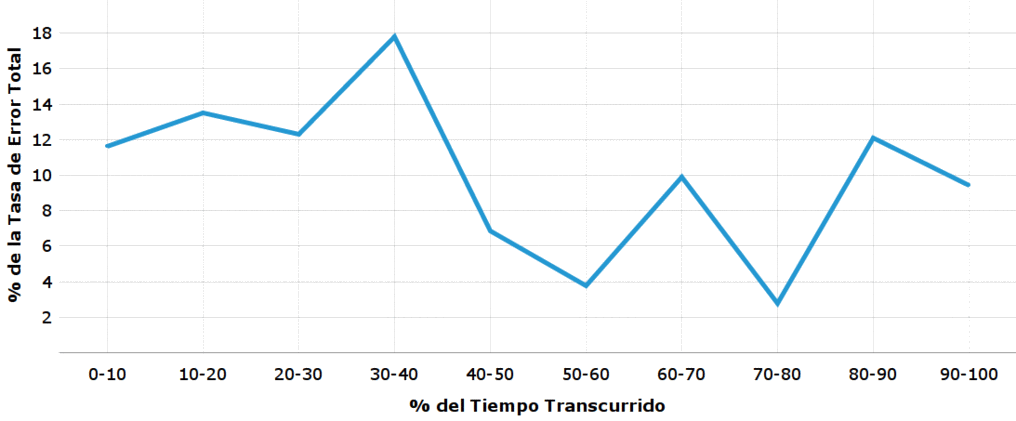
\includegraphics[width=1\linewidth]{./graphics/error_tiempo.png}
\caption{Distribuci\'on del error humano por etapas de la sesi\'on.}
\label{figure:gerror-tiempo}
\end{figure}
\end{columns}

\end{frame}

\begin{frame}{Resultados Obtenidos}
\framesubtitle{Encuesta}
\begin{columns}
\column{0.35\linewidth}
\begin{table}[H] 
\centering
\tiny
\begin{tabular}{|r|r|r|r|r|}
\hline
            & Promedio \\
\hline
Vocabulario    & 6.17 \\
Comandos    & 6.58 \\
Entrenamiento  & 6.25 \\
Interfaz por Voz & 5.83 \\
\hline
\end{tabular}
\caption{Resumen de la encuesta realizada.}
\label{sec:tabla-encuesta}
\end{table}
\column{0.65\linewidth}
\begin{figure}[ht]
\centering
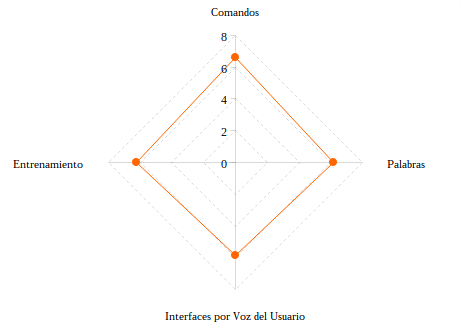
\includegraphics[width=1\linewidth]{./graphics/kiviat0.png}
\caption{Gr\'afico radial resumen de la encuesta realizada.}
\label{figure:kiviat-encuesta1}
\end{figure}
\end{columns}
\end{frame}

\begin{frame}{Resultados Obtenidos}
\framesubtitle{Encuesta}
\begin{columns}
\column{0.35\linewidth}
\begin{table}[H] 
\centering
\tiny
\begin{tabular}{|r|r|r|r|r|}
\hline
            & Promedio \\
\hline
Vocabulario    & 0.45 \\
Comandos    & 0.86 \\
Entrenamiento  & 0.55 \\
Interfaz por Voz & 0.5 \\
\hline
\end{tabular}
\caption{Resumen de la encuesta realizada. Valores reescalados.}
\label{sec:tabla-encuesta-normalizada}
\end{table}
\column{0.65\linewidth}
\begin{figure}[ht]
\centering
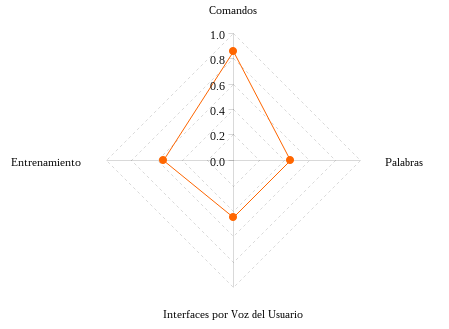
\includegraphics[width=1\linewidth]{./graphics/kiviat.png}
\caption{Gr\'afico radial resumen de la encuesta realizada. Valores reescalados.}
\label{figure:kiviat-encuesta2}
\end{figure}
\end{columns}
\end{frame}
\section{Conclusiones}

\begin{frame}{Conclusiones (1/3)}
\framesubtitle{Dise\~no e Implementaci\'on}
\vspace{-0.5cm}
\begin{table}[ht]
  \begin{tabular}{|p{2.75cm}|p{8cm}|}
    \hline
    Tema & Conclusi\'on \\
    \hline
    \multirow{3}{2.75cm}{\uncover<2-7>{\textbf{Dise\~no de la Interfaz}}} & \uncover<2-7>{La naturalidad del lenguaje es de gran importancia \mbox{para la interfaz.}} \\
    \hhline{~-}
    &\uncover<3-7>{Interactuar con la aplicaci\'on, no con la interfaz \mbox{gr\'afica.}}\\
    \hhline{~-}
    &\uncover<4-7>{Utilizar el sonido como medio de \mbox{retroalimentaci\'on.}} \\
    \thickhline
    \multirow{3}{2.75cm}{\uncover<5-7>{\textbf{Implementaci\'on de la Interfaz}}} & \uncover<5-7>{Evaluar las herramientas de reconocimiento del \mbox{habla} disponibles.}\\
    \hhline{~-}
    & \uncover<6-7>{Considerar la integraci\'on del motor de \mbox{reconocimiento} y la aplicaci\'on.} \\
    \hhline{~-}
    & \uncover<7-7>{Realizar pruebas con usuarios para perfeccionar la interacción.}\\
    \hline
  \end{tabular}
\end{table}


% \begin{itemize}
%     \item Dise\~no de la Interfaz
%         \begin{itemize}
%             \item La naturalidad del lenguaje es de gran importancia para la interfaz.
%             \item Interactuar con la aplicaci\'on, no con la interfaz gr\'afica.
%             \item Utilizar el sonido como medio de retroalimentaci\'on.
%         \end{itemize}
%     \item Implementaci\'on de la Interfaz
%         \begin{itemize}
%             \item Seleccionar las herramientas de acuerdo al \mbox{proyecto}.
%             \item Considerar la posibilidad de errores en el \emph{software}.
%             \item Realizar pruebas y modificaciones tempranas.
%         \end{itemize}
% \end{itemize}

\end{frame}

\begin{frame}{Conclusiones (2/3)}
\framesubtitle{Prueba con Usuarios}
\vspace{-0.5cm}
\begin{table}[ht]
  \begin{tabular}{|p{2cm}|p{8.5cm}|}
    \hline
    Tema & Conclusi\'on \\
    \hline
    \multirow{3}{2cm}{\uncover<2-8>{\textbf{Correlaci\'on}}} & \uncover<2-8>{Errar es humano: Los usuarios prefieren probar \mbox{(y fallar) a leer.}} \\
    \hhline{~-}
    &\uncover<3-8>{Considerar la memoria del usuario al evaluar los \mbox{resultados.}}\\
    \hhline{~-}
    &\uncover<4-8>{Validar hip\'otesis triviales.}\\
    \thickhline
    \multirow{5}{2cm}{\uncover<5-8>{\textbf{Error Humano}}} & \uncover<5-8>{Evitar comandos de m\'as de 4 palabras.}\\
    \hhline{~-}
    & \uncover<6-8>{Dar la debida importancia al entrenamiento del \mbox{usuario.}}\\
    \hhline{~-}
    & \uncover<7-8>{Considerar factores humanos como la fatiga.}\\
    \hhline{~-}
    & \uncover<8-8>{Reconsiderar los comandos con tasa de error elevada.}\\
    \hline
  \end{tabular}
\end{table}

% \begin{itemize}
%     \item Correlaci\'on
%         \begin{itemize}
%             \item Errar es humano: Los usuarios prefieren probar (y fallar) a leer.
%             \item Considerar la memoria del usuario al evaluar los resultados.
%             \item Validar hip\'otesis triviales.
%         \end{itemize}
%     \item Error Humano
%         \begin{itemize}
%             \item Evitar comandos de m\'as de 4 palabras.
%             \item El contexto de los comandos no es lo (\'unico) que importa.
%             \item Dar la debida importancia al entrenamiento del usuario.
%             \item Considerar factores humanos como la fatiga.
%             \item Reconsiderar los comandos con tasa de error elevada.
%         \end{itemize}
%     \item Encuesta
%         \begin{itemize}
%             \item Opini\'on positiva de los usuarios hacia \emph{TamTam Listens} y el reconocimiento del habla.
%             \item Los puntos a mejorar est\'an en las respuestas de los usuarios.
%             \item Preferir aplicaciones poco interactivas para interfaces por voz.
%         \end{itemize}
%     \end{itemize}

\end{frame}

\begin{frame}{Conclusiones (3/3)}
\framesubtitle{Prueba con Usuarios}
\vspace{-0.5cm}
\begin{table}[ht]
  \begin{tabular}{|p{2cm}|p{8.5cm}|}
    \hline
    Tema & Conclusi\'on \\
    \hline
    \multirow{3}{2cm}{\uncover<2-4>{\textbf{Encuesta}}} & \uncover<2-4>{Opini\'on positiva de los usuarios hacia \mbox{\emph{TamTam Listens} y el reconocimiento del habla.}}\\
    \hhline{~-}
    & \uncover<3-4>{Los puntos a mejorar est\'an en las respuestas de los usuarios.}\\
    \hhline{~-}
    & \uncover<4-4>{Preferir aplicaciones poco interactivas para interfaces por voz.}\\
    \hline
  \end{tabular}
\end{table}
\end{frame}
\section{Trabajos Futuros}

\begin{frame}{Trabajos Futuros}

\begin{itemize}
    \item Utilizar TamTam Listens con personas con discapacidad.
    \item Modelo Ac\'ustico Localizado.
    \item Reducci\'on de ruido.
    \item Optimizar generaci\'on de Modelo Ac\'ustico.
    \item Integraci\'on con otros proyectos.
\end{itemize}

\end{frame}


%%% BIBLIOGRAFIA %%%
\begin{frame}[allowframebreaks]
\frametitle{Referencias}
\printbibliography
\end{frame}



\end{document}
